\documentclass{article}
\usepackage{graphicx}
\usepackage[letterpaper,body={6.1in,9in},top=.8in,left=1.2in]{geometry}
\usepackage[no-math]{fontspec}
\usepackage{verbatim,fancyvrb}
\usepackage{gretl}
%\usepackage{amsmath}
\usepackage[authoryear]{natbib}
\usepackage{hyperref}

\setmonofont{DejaVu Sans Mono}[Scale=0.9]

\setlength{\parindent}{0pt}
\setlength{\parskip}{1ex}

\hypersetup{pdftitle={ETS 1.0},
            pdfauthor={Allin Cottrell and Ignacio Díaz-Emparanza},
            colorlinks=true,
            linkcolor=blue,
            urlcolor=red,
            citecolor=steel,
            bookmarksnumbered=true,
            plainpages=false
}

\begin{document}

\begin{center}
  {\Large \textbf{ETS 1.0}} \\[6pt]
  Allin Cottrell and Ignacio Díaz-Emparanza \\[6pt]
  2026-11-01
\end{center}

\section{Introduction}
\label{sec:intro}

This package implements exponential smoothing for time series, in three
variants:
\begin{enumerate}
\item \textit{Simple} exponential smoothing: a level component only.
\item \textit{Holt's} method \citep{holt57}, also known as double
  exponential smoothing: level and trend components.
\item The \textit{Holt-Winters} method \citep{winters60}, also known as
  triple exponential smoothing: level, trend and seasonal components,
  where the seasonal component can be either additive or multiplicative.
\end{enumerate}
It requires time-series data. The seasonal variants require data with a
seasonal dimension; quarterly or monthly data are the best bet for
suitability. Daily or hourly data might be suitable, subject to the
qualifications noted in section~\ref{sec:daily}. Weekly seasonality is
not supported: it's too complicated.

The package combines and supersedes the earlier \textsf{Holt} and
\textsf{Winters} packages, and adds simple exponential smoothing for
completeness. See section~\ref{sec:update} for an account of the
differences from those packages. The earlier versions of \textsf{Holt}
(1.0, 2015) and \textsf{Winters} (1.1, 2022) were written by Ignacio
Díaz-Emparanza; the versions 2.\textit{n} on which this package builds
were written by Allin Cottrell. Most of the work on the consolidated
\textsf{ETS} package was done by Claude Sonnet 5.5. (\textsf{ETS} can be
thought of as indicating ``Exponential Time-series Smoothing'' or
``Error, Trend, Seasonal''.)

\subsection{The recursions}

The filtering recursions and forecasting equations are shown below. The
notation is based on \citet[chapter 8]{hyndman2021}: $\ell$ denotes the
level, $b$ the trend or slope, and $s$ the seasonal; $\alpha$, $\beta$
and $\gamma$ are the respective smoothing parameters. In addition $m$
denotes the periodicity of the data (gretl's \verb|$pd|) and $k$ is the
integer part of $(h-1)/m$ ($=0$ when $h=1$).

\textit{Simple}:
\begin{align*}
  \ell_t &= \alpha y_t + (1-\alpha) \ell_{t-1}\\
  \hat{y}_{t+h|t} &= \ell_t
\end{align*}

\textit{Holt}:
\begin{align*}
  \ell_t &= \alpha y_t + (1-\alpha) (\ell_{t-1} + b_{t-1})\\
  b_t &= \beta (\ell_t - \ell_{t-1}) + (1-\beta) b_{t-1}\\
  \hat{y}_{t+h|t} &= \ell_t + hb_t
\end{align*}

\textit{Holt-Winters, additive}:
\begin{align*}
  \ell_t &= \alpha (y_t - s_{t-m}) + (1-\alpha) (\ell_{t-1} + b_{t-1})\\
  b_t &= \beta (\ell_t - \ell_{t-1}) + (1-\beta) b_{t-1}\\
  s_t &= \gamma (y_t - \ell_t) + (1-\gamma) s_{t-m}\\
  \hat{y}_{t+h|t} &= \ell_t + hb_t + s_{t+h-m(k+1)}
\end{align*}

\textit{Holt-Winters, multiplicative}:
\begin{align*}
  \ell_t &= \alpha (y_t / s_{t-m}) + (1-\alpha) (\ell_{t-1} + b_{t-1})\\
  b_t &= \beta (\ell_t - \ell_{t-1}) + (1-\beta) b_{t-1}\\
  s_t &= \gamma\, y_t / \ell_t + (1-\gamma) s_{t-m}\\
  \hat{y}_{t+h|t} &= (\ell_t + hb_t)\, s_{t+h-m(k+1)}
\end{align*}

\subsection{Sample ranges and forecasts}

Like most functions in gretl, \texttt{ETS} confines its operations
to the sample range in force when the function is called. We'll refer
to the (1-based) start and end of this range as $t_1$ and $t_2$,
respectively.\footnote{This range can be set via the \texttt{smpl}
  command. If \texttt{smpl} has not been invoked since a dataset was
  opened $t_1$ will equal 1 and $t_2$ will equal the total number of
  observations.}  In addition, let $T$ denote the date of the last
valid observation of the variable to be predicted, $y$.

There are two cases to be considered:
\begin{enumerate}
\item $T < t_2$: in this case there's a `tail' of observations for
  which values of $y_t$ are not available.  \texttt{ETS} will by
  default produce predictions for these observations.
\item $T = t_2$: there's no tail for genuine out-of-sample prediction,
  but you can specify a number of observations, \texttt{ntest}, to
  reserve for pseudo-out-of-sample prediction. In that case the
  training recursion will be terminated at observation $T-$
  \texttt{ntest}.
\end{enumerate}

If you want case 1 but your dataset doesn't contain any extra trailing
observations it's straightforward to add them using the
\texttt{dataset addobs} command, or via the \textsf{Add observations}
item under the \textsf{Data} menu in the graphical interface.

Conversely, if the dataset does contain extra trailing observations
but you want case 2, specifying a positive value for \texttt{ntest}
will result in the extra observations being ignored and
pseudo-out-of-sample forecasts being produced.

\section{The public functions}
\label{sec:public}

The primary function has the following signature:
\begin{nscode}
function bundle ETS (const series y, const bundle specs[null])
\end{nscode}

The required argument \texttt{y} specifies the series to be processed.
The second argument---which can be omitted, as indicated by the
\texttt{null} modifier---may contain one or more of the following
options:

\begin{itemize}
\item \texttt{trend} (integer): 0 or 1, to exclude or include a trend
  component. The default is 0, unless \texttt{seasonal} is non-zero, in
  which case it is 1.
\item \texttt{seasonal} (integer): 0 for no seasonal component (the
  default), 1 for an additive seasonal component or 2 for a
  multiplicative one. A seasonal component requires a trend: setting
  \texttt{seasonal} non-zero along with \texttt{trend} = 0 is an error.
\item \texttt{theta} (matrix): if supplied, this must be a vector
  holding the smoothing parameters, each in $[0,1]$. The length depends
  on the model: 1 for simple smoothing, $\theta = (\alpha)$; 2 for Holt,
  $\theta = (\alpha, \beta)$; and 3 for Holt-Winters,
  $\theta = (\alpha, \beta, \gamma)$. If \texttt{theta} is not given the
  parameters are determined automatically.
\item \texttt{init} (matrix): if supplied, this must be a vector
  holding the initial state: the level, followed by the trend if
  applicable, followed by the $m$ seasonals (oldest first) if
  applicable, where $m$ is the periodicity of the data. The length is
  thus 1 for simple smoothing, 2 for Holt and $m+2$ for Holt-Winters.
  In the multiplicative case the level and seasonals must be positive.
  If \texttt{init} is given it is held fixed: it is neither estimated
  nor overwritten, and if \texttt{theta} is not given only the smoothing
  parameters are optimized. This is mainly useful for testing and for
  replicating results from other software.
\item \texttt{ntest} (integer): specifies the number of
  observations at the end of the range of \texttt{y} values to reserve
  for testing via pseudo-out-of-sample forecasting. The default value
  is 0.
\item \texttt{verbose} (integer): controls the verbosity of output, with
  levels 0, 1 (the default), 2 or 3.
\end{itemize}

Thus the model is selected by the combination of \texttt{trend} and
\texttt{seasonal}:
\begin{center}
  \begin{tabular}{ccl}
    \textit{trend} & \textit{seasonal} & \textit{model} \\[3pt]
    0 & 0 & simple exponential smoothing \\
    1 & 0 & Holt \\
    1 & 1 & Holt-Winters, additive \\
    1 & 2 & Holt-Winters, multiplicative
  \end{tabular}
\end{center}

The return value from \texttt{ETS} is a bundle containing the
following elements:
\begin{itemize}
\item \texttt{theta}: a vector holding the smoothing parameter values.
\item \texttt{init}: a vector holding the initial state: the level,
  followed by the trend if applicable, followed by $m$ seasonals if
  applicable.
\item \texttt{trend}, \texttt{seasonal}: the model flags as described
  above.
\item \texttt{ntest}: a non-negative integer indicating how many
  observations were reserved for pseudo-out-of-sample forecasting.
\item \texttt{S}: a matrix with a row for each observation in the range
  from $t_1$ to the last forecast. Column 1 holds the data passed as
  \texttt{y}; the next columns hold the estimated level, then the trend
  (if applicable), then the seasonal (if applicable); and the final
  column holds forecasts. Columns are named. More details on this matrix
  are provided below.
\item \dtk{RMSE_train}: the root mean squared error for the 1-step
  ahead forecasts made using the training data.
\item \dtk{MAE_train}: the mean absolute error for the 1-step
  ahead forecasts made using the training data.
\item \texttt{yname}: the name of the input series.
\item \texttt{limits}: a 3-vector holding the 1-based indices of the
  first training observation, the last training observation, and the
  last forecast. If there are no post-training forecasts (testing or
  out-of-sample) the third element is equal to the second.
\item \texttt{nparms}: the number of estimated parameters (smoothing
  parameters plus free elements of the initial state), used in
  calculating degrees of freedom for confidence intervals.
\end{itemize}
If \texttt{ntest} is non-zero, two additional items are included in the
bundle, namely the RMSE and MAE for the pseudo-out-of-sample forecasts,
under the keys \dtk{RMSE_test} and \dtk{MAE_test}.

If any post-training forecasts are performed (either in response to
\texttt{ntest} or out of sample) and the model is not multiplicative,
the matrix \texttt{S} acquires a further column, holding standard errors
for these forecasts. (In the multiplicative case there is no closed
form for the forecast variance; see below.)

A simple \textit{plotting} function is also supplied:
\begin{nscode}
function void ETS_plot (bundle *b, int ptype, matrix ci_levels[null])
\end{nscode}
The first argument should be a pointer to a bundle obtained from
\texttt{ETS} and the second argument should be either 1 for a plot of
actual and forecast values, or 2 for a plot of the components: level;
trend and seasonal if applicable; and irregular. The third (optional)
argument is referenced only when \texttt{ptype} = 1 and post-training
forecasts have been performed, in which case confidence intervals will be
shown. If \dtk{ci_levels} is supplied it must be a 2-vector holding two
distinct confidence levels, in percentage form and in the range 50 to
99. If this argument is not given the levels default to 80\% and 95\%.
For the additive models the intervals are based on analytical standard
errors. In the multiplicative case they are simulation-based, using 10000
iterations of draws from the $t(\nu)$ distribution, where $\nu$ equals
the number of training observations minus the number of parameters
being estimated.

A third public function is available when, and only when, post-training
forecasts are generated:
\begin{nscode}
function matrix ETS_ci_matrix (const bundle b, matrix ci_levels[null])
\end{nscode}
The argument must be a bundle obtained from \texttt{ETS}. The return
value is a matrix with four columns, and rows equal to the number of
post-training forecasts. By default the first two columns hold the lower
and upper limits for an 80 percent \textit{confidence interval} and the
second two hold the limits for a 95 percent interval. The optional
\dtk{ci_levels} argument works just as with \dtk{ETS_plot}, and the
intervals are calculated as described above.

\section{Command-line usage}
\label{sec:auto}

We'll illustrate with replication of three examples from
\citet{hyndman2021}. First, simple exponential smoothing applied to
Algerian exports (section 8.1):
\begin{nscode}
include ETS.gfn
open alg_exports.gdt --frompkg=ETS
dataset addobs 5
bundle sb = ETS(Exports)
ETS_plot(&sb, 1)
\end{nscode}

The \dtk{alg_exports} dataset contains 58 annual observations from
1960 to 2017, which are used for training the model. The five added
observations, 2018 to 2022, are then used for out-of-sample
forecasting. Since \texttt{theta} is not specified, both $\alpha$ and
the initial level will be optimized automatically; see
section~\ref{sec:details} for details. Second, Holt's method applied to
Australian population (section 8.2):
\begin{nscode}
open auspop.gdt --frompkg=ETS
dataset addobs 10
bundle hb = ETS(pop, _(trend=1))
ETS_plot(&hb, 1)
ETS_plot(&hb, 2)
\end{nscode}
And third, the Holt-Winters method (multiplicative variant) applied to
Australian tourism (section 8.3):
\begin{nscode}
open aus_holidays.gdt --frompkg=ETS
dataset addobs 12
bundle wb = ETS(Trips, _(seasonal=2))
ETS_plot(&wb, 1)
ETS_plot(&wb, 2)
\end{nscode}
The \dtk{aus_holidays} dataset contains 80 quarterly observations
from 1998:1 to 2017:4; the twelve added observations are for
out-of-sample forecasting.

One might choose, instead, to use the \texttt{ntest} option to get
\texttt{ETS} to generate (say) eight pseudo-out-of-sample forecasts:
\begin{nscode}
open aus_holidays.gdt --frompkg=ETS
bundle wb = ETS(Trips, _(seasonal=2, ntest=8))
\end{nscode}
This generates forecasts for 2016:1 to 2017:4, and the RMSE and MAE for
these testing forecasts are printed.

\section{Output details}
\label{sec:out}

Table~\ref{tab:verbose} shows what is printed by \texttt{ETS} as a
function of the \texttt{verbose} option. Examples of the table of
results displayed when \texttt{verbose} is 1 or greater are presented
in listings~\ref{list:results1} and~\ref{list:results2}. The matrix
\texttt{S} that's included in the bundle returned by \texttt{ETS} is
basically a matrix version of this table. If you want to grab the
columns of \texttt{S} as a list of series you can do something like
this:
\begin{nscode}
bundle sb = ETS(Exports)
list L = mat2list(sb.S)
list L print # show all the series in L
\end{nscode}

\begin{table}[htbp]
  \caption{Effect of the verbose option}
  \label{tab:verbose}
  \begin{tabular}{cp{4.5in}}
    \textit{verbose} & \textit{cumulative effect} \\[6pt]
    0 & Nothing is printed. \\
    1 & Parameters and initializer are reported, also a table
        of results (see below) and the SSE, RMSE and MAE for the
        training data.\\
    2 & If optimization is performed, partial information on
        progress of the iterative procedure is shown. \\
    3 & If optimization is performed, progress of the
        optimizer is shown in full.
  \end{tabular}
\end{table}

\begin{script}[htbp]
  \caption{Partial listing of results from the simple exponential
    smoothing example in Section~\ref{sec:auto}.}
  \label{list:results1}
\begin{code}
Simple exponential smoothing
Training range: 1960 to 2017
Out-of-sample forecast: 2018 to 2022

automatic parameter values:
  α = 0.839783

estimated initializer:

level       39.538

training SSE = 1995.29, RMSE = 5.86528, MAE = 4.00111

                y        level     forecast

1960     39.04317     39.12248     39.53815
1961     46.24456     45.10348     39.12248
1962     19.79387     23.84890     45.10348
1963     24.68468     24.55078     23.84890
...
2014     30.21912     30.80023     33.84617
2015     23.17178     24.39399     30.80023
2016     20.86001     21.42621     24.39399
2017     22.63889     22.44460     21.42621
2018                               22.44460
2019                               22.44460
2020                               22.44460
2021                               22.44460
2022                               22.44460
\end{code}
\end{script}

\begin{script}[htbp]
  \caption{Partial listing of results from the Holt-Winters example in
    Section~\ref{sec:auto}: forecasts for 2018:1 and beyond are
    out-of-sample.}
  \label{list:results2}
\begin{code}
Holt-Winters, using multiplicative formula
Training range: 1998:1 to 2017:4
Out-of-sample forecast: 2018:1 to 2020:4

automatic parameter values:
  α = 0.246678, β = 0.122928, γ = 0

estimated initializer:

level       9.9096
trend    -0.028539
seas1       1.1626
seas2      0.96686
seas3      0.92687
seas4      0.94364

training SSE = 13.4951, RMSE = 0.410718, MAE = 0.307344

                  y        level        trend     seasonal     forecast

1998:1     11.80604      9.94851     -0.02025     1.162641     11.48812
1998:2      9.27566      9.84571     -0.03040     0.966858      9.59922
1998:3      8.64249      9.69423     -0.04528     0.926865      9.09748
1998:4      9.29952      9.69977     -0.03903     0.943636      9.10509
...
2017:1     12.40642     10.79711      0.08755     1.162641     12.60121
2017:2     10.47120     10.87121      0.08590     0.966858     10.52392
2017:3     10.49917     11.04850      0.09713     0.926865     10.15576
2017:4     11.21082     11.32689    0.1194143     0.943636     10.51742
2018:1                                                         13.30794
2018:2                                                         11.18241
2018:3                                                         10.83055
2018:4                                                         11.13920
...
\end{code}
\end{script}

If the bundle includes the forecast standard errors (additive models
with post-training forecasts) the final column of \texttt{S} is named
\texttt{stderr}. If gretl is version 2026c or later the bundle also
contains ``virtual series'' named after the input series: for a series
\texttt{y}, \dtk{y_level}, \dtk{y_fcast} and \dtk{y_irreg},
plus \dtk{y_trend} and \dtk{y_season} where applicable.

\section{GUI usage}
\label{sec:gui}

When you install this package you should get the option of attaching it
as the menu item \textsf{Variable/Filter} in gretl's main
window. Clicking this item brings up a dialog box in which you choose
the model (simple, Holt, or Holt-Winters additive or multiplicative),
whether the smoothing parameters are to be estimated or pre-specified,
the number of test observations and the verbosity level.

\begin{figure}[htpb]
  \centering
  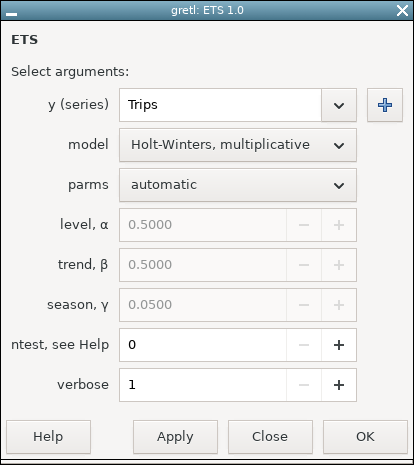
\includegraphics[scale=0.60]{ETS_dialog.png}
  \caption{ETS dialog, under the Variable/Filter menu}
  \label{fig:dialog}
\end{figure}

\begin{figure}[p]
  \centering
  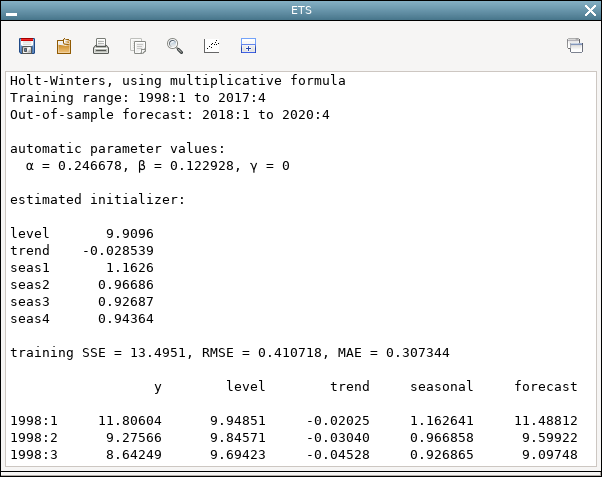
\includegraphics[scale=0.60]{output_window.png}
  \caption{ETS output window}
  \label{fig:output}
\end{figure}

Clicking the \textsf{Help} button will bring up a brief explanation of
each control. Only those smoothing parameters relevant to the selected
model are used when they are pre-specified: $\alpha$ for simple
smoothing, $\alpha$ and $\beta$ for Holt, all three for Holt-Winters.
On clicking \textsf{OK} you should get a window showing the results. The
toolbar at the top of this window includes a \textsf{Graph} button which
gives access to two types of plot, one showing actual and forecast
\texttt{y} and one showing the components.

\section{Technical details}
\label{sec:details}

This section offers some details on the initialization with which the
recursions are started, the optimization that is carried out if
\texttt{theta} is not given by the caller, and the calculation of
forecast standard errors.

\subsection{Initialization}

Let $\tau$ denote the first period in which $y$ is observed. For the
non-seasonal models the basic initialization is as follows.
\begin{itemize}
\item The initial level, $\ell_{\tau-1}$, is set to the first observed
  value $y_{\tau}$.
\item In the Holt case the initial trend, $b_{\tau-1}$, is set to the
  first observed difference, $y_{\tau+1} - y_{\tau}$.
\end{itemize}

For the seasonal models the rule-of-thumb is calculated as per the
suggestion in \cite{hyndman98}, which is also described in
\cite{hyndman2010}.
\begin{itemize}
\item The initial level, $\ell_{\tau-1}$, is set to the mean of the
  $m$ values $y_{\tau}, y_{\tau+1},\dots, y_{\tau+m-1}$.
\item The initial trend, $b_{\tau-1}$, is set to the mean of the
  first $m$ seasonal differences:
 \[
    m^{-1} \sum_{i=0}^{m-1} \left(y_{\tau+i+m} - y_{\tau+i}\right)
 \]
\item The initial seasonals are then set to the ratio of period-specific
  $y_t$ to $\ell_{\tau-1}$ for the first $m$ observations
  (multiplicative case) or the difference between $y_t$ and
  $\ell_{\tau-1}$ (additive case).
\end{itemize}

\subsection{Optimization}

Two cases arise.
\begin{itemize}
\item If \texttt{theta} is not specified, the parameter values and
  initializer are optimized, with the criterion of minimizing the sum of
  squared one-step ahead forecast errors for the training range. The
  starting point for the parameters is
  $\alpha = \beta = 0.5, \gamma = 0.05$ (as applicable). Optimization is
  performed using the L-BFGS algorithm (see the chapter on Numerical
  methods in the \GUG\ for details), with the smoothing parameters
  constrained to lie in $[0,1]$.

  In the additive models (simple, Holt and additive Holt-Winters) the
  recursion is linear in the state, so given the smoothing parameters
  the one-step forecasts are linear in the initial state; the
  initializer can therefore be concentrated out and solved for by OLS
  within each evaluation of the criterion, and L-BFGS need only search
  over the smoothing parameters.\footnote{Thanks go to Jack Lucchetti for
    suggesting a particularly efficient approach to the optimization,
    making use of gretl's \texttt{varsimul} function.} In the seasonal
  case the seasonals are constrained to sum to zero, since the initial
  level and the seasonal mean are not separately identified. In the
  multiplicative case the initializer is optimized jointly with the
  smoothing parameters via L-BFGS, starting from the rule-of-thumb
  values, with the seasonals normalized to average 1.
\item If \texttt{theta} is given, the treatment of the initializer
  depends on the model. For the seasonal models, it is optimized
  conditional on $\theta$, using the same criterion: in the additive
  case this is a linear least-squares problem with a closed-form
  solution, while in the multiplicative case L-BFGS is used. For the
  non-seasonal models the initializer is just the basic value
  described above; no optimization is performed.
\item If \texttt{init} is given (with or without \texttt{theta}) it is
  used as is, and only the smoothing parameters, if not given, are
  optimized (by L-BFGS, for all four models). The supplied seasonals
  are not renormalized, so the \texttt{init} in the returned bundle
  is exactly what was passed in.
\end{itemize}

\subsection{Forecast standard errors}

For the additive models, the $h$-step ahead forecast error variance
follows \citet[section 8.7]{hyndman2021}:
\[
  \sigma^2_h = \sigma^2 \left[ 1 + \sum_{j=1}^{h-1} c_j^2 \right],
  \quad c_j = \alpha + \beta^{*} j + \gamma^{*}\, I(j \bmod m = 0),
\]
where $\sigma^2$ is estimated by the MSE for the training data and
$\beta^{*} = \alpha\beta$ and $\gamma^{*} = (1-\alpha)\gamma$ are the
trend and seasonal parameters of the equivalent ETS(A,$\cdot$,$\cdot$)
model (see \citealt[sections 8.3 and 8.5]{hyndman2021}). Terms that do not
apply to the model in question ($\beta^{*}$ in the simple case,
$\gamma^{*}$ in the non-seasonal cases) are zero. These expressions
reduce to the familiar closed forms: for simple smoothing,
$\sigma^2[1 + (h-1)\alpha^2]$, and for Holt,
\[
  \sigma^2_h = \sigma^2 \left[ 1 + (h-1) \{\alpha^2 + \alpha\beta^{*} h
        + \frac{1}{6} \beta^{*2}h(2h-1) \} \right].
\]
The intervals use quantiles of the $t(\nu)$ distribution, with $\nu$
equal to the number of training observations minus the number of
estimated parameters (smoothing parameters plus free initial-state
elements; this is the \texttt{nparms} element of the returned bundle).

\section{Daily and hourly data}
\label{sec:daily}

As mentioned in section~\ref{sec:intro} the seasonal models may be
applicable to daily data, with $m$ = 5, 6 or 7 days per week. In this
context `seasonality' means intra-week variability. However, the results
will be meaningful only if the data are `complete', in the sense that
each week in the sample range includes $m$ valid daily observations. It
should go without saying that financial market data, even if complete,
are unlikely to be suitable since seasonal variation would be a clear
violation of market efficiency (in the narrow sense in which market
efficiency is a plausible hypothesis).

Gretl also supports hourly data ($m=24$) and the seasonal models may work
if there's seasonality in the form of intra-day variability. Again,
however, the series in question has to be complete over the given sample
range.

\section{Comparison with Holt and Winters}
\label{sec:update}

ETS replaces the separate \textsf{Holt} (2.0) and \textsf{Winters}
(2.3) packages. For users of those packages the principal changes are
these.
\begin{itemize}
\item There is a single primary function, \texttt{ETS()}. The call
  \texttt{Holt(y, specs)} becomes \texttt{ETS(y, \_(trend=1, \dots))}
  while \texttt{Winters(y, \_(additive=1, \dots))} becomes
  \texttt{ETS(y, \_(seasonal=1, \dots))} and
  \texttt{Winters(y, \_(additive=0, \dots))} becomes
  \texttt{ETS(y, \_(seasonal=2, \dots))}. Note that \texttt{Winters}
  defaulted to the multiplicative variant; \texttt{ETS} requires you to
  say which seasonal variant you want.
\item The plotting function is now \dtk{ETS_plot}.
  Confidence intervals are available via
  \dtk{ETS_ci_matrix}, which is new for the seasonal models and
  covers both the additive and multiplicative cases.
\item The results matrix in the returned bundle is named \texttt{S}, in
  place of \texttt{H} (Holt) or \texttt{W} (Winters). Its columns are as
  before except that columns which do not apply to the model are
  omitted and the columns are named. In particular, the forecast is
  the last column other than the standard errors (column 4 for Holt, 5
  for Holt-Winters); the virtual series keep the same suffixes as before.
\item The bundle also contains the model flags \texttt{trend} and
  \texttt{seasonal} (replacing \texttt{additive}) and \texttt{nparms}.
\item For the same model, parameters and options, the numerical results
  are the same as from the earlier packages (up to the tolerance of the
  optimizer). The forecast standard errors for the additive models are
  also identical.
\item The \dtk{ETS_gui} dialog offers a single \textsf{model}
  selector in place of the \textsf{formula} selector in the
  \textsf{Winters} dialog.
\end{itemize}

\section{Change log}
\label{sec:log}

\begin{itemize}
\item \texttt{v1.0}, 2026-11-01: Initial release, combining the
  \textsf{Holt} 2.0 and \textsf{Winters} 2.3 packages and adding simple
  exponential smoothing.
\item \texttt{v1.1}: Added the \texttt{init} option; the
  \texttt{nparms} count now excludes fixed parameters.
\end{itemize}

\bibliographystyle{gretl}
\bibliography{gretl}

\end{document}
